\chapter{Experiments}

\section{Classical Computer Vision-based Approach}
\subsection{The General Scheme}
Here
\begin{figure}
    \centering
    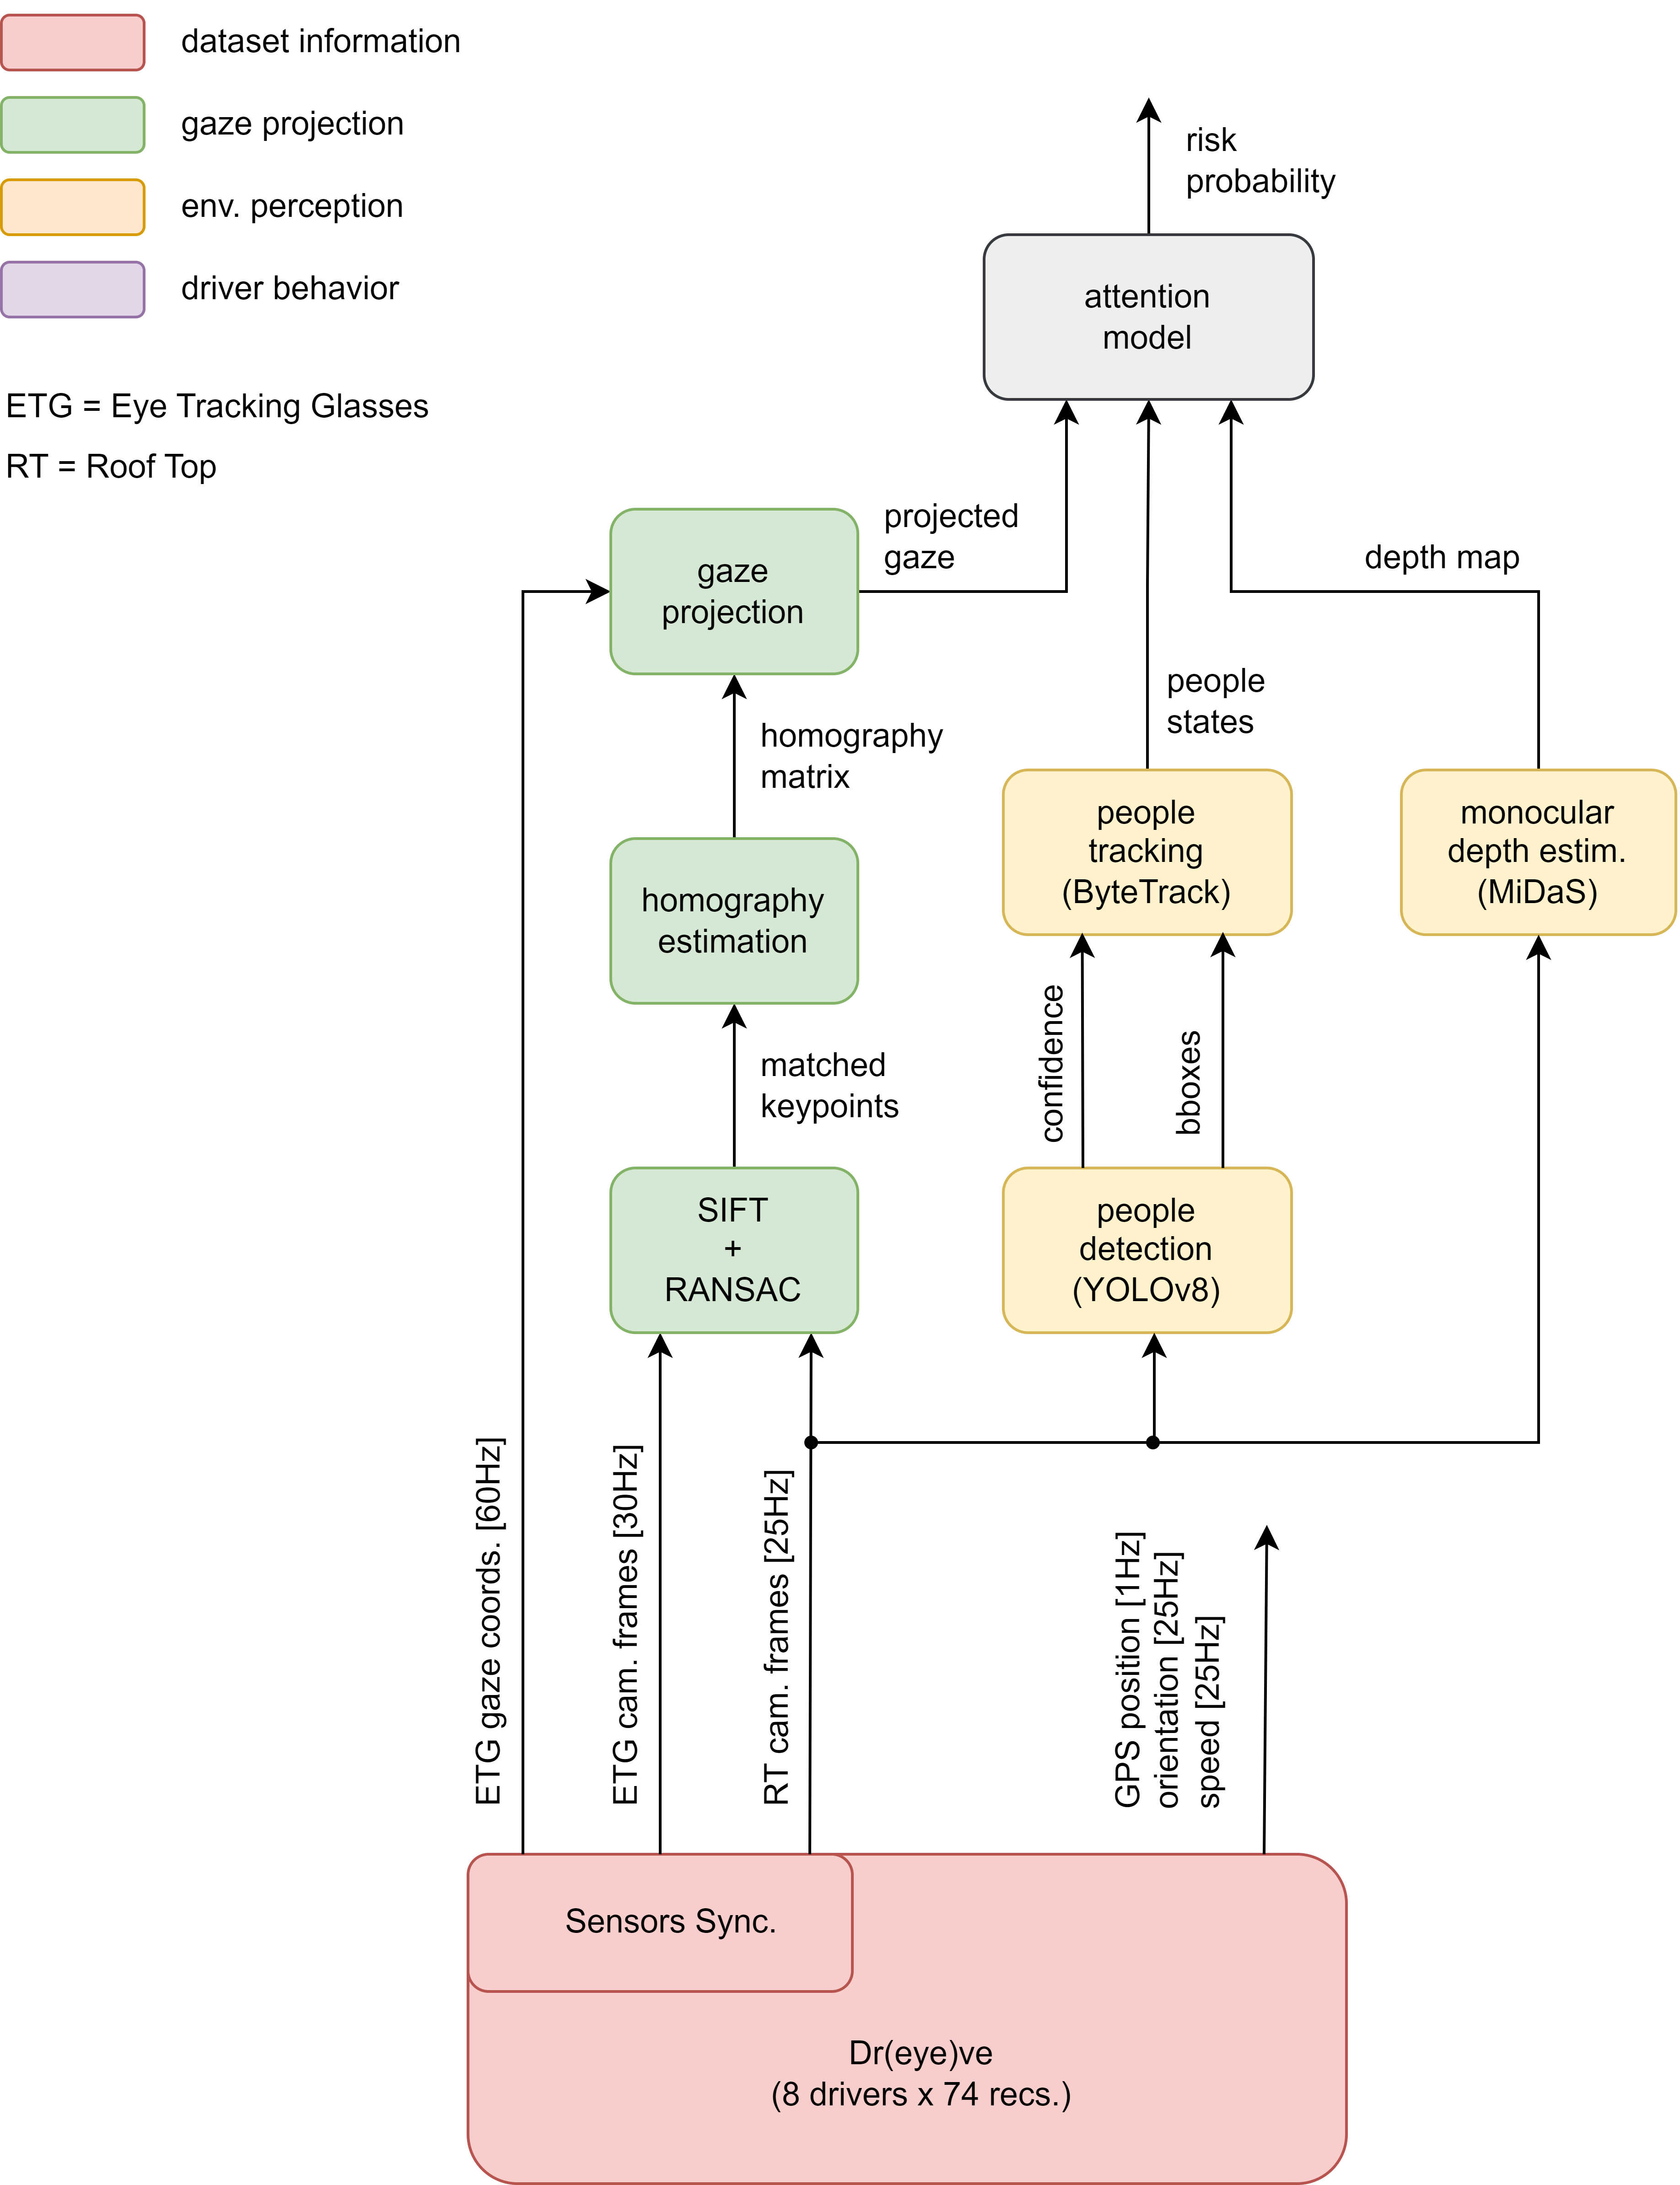
\includegraphics[width=0.95\textwidth]{images/dreyeve/classic_scheme.png}
    \vspace*{0.6cm}
    \caption{The overall driver's attention scheme. It is divided into four main 
    stages: data synchronization, homography projection of the gaze, scene 
    perception and the driver's behavioral model.
    }
    \label{fig:driver_attention}
\end{figure}
\subsection{Data Preprocessing}
\subsection{Gaze Projection}
\subsection{Distribution of People in Dr(eye)ve}

\subsection{Targets Data Representation}

\subsection{Gaze Interaction with Targets}

\subsection{Adding Depth Information}

\subsection{Adding Spatial Information}


\section {Deep Learning-based Approach}
\subsection{The General Scheme}
\subsection{The Artificial Bias}
\subsection{Data Preprocessing of Dr(eye)ve}
\subsection{Supervised Training on Dr(eye)ve}
\subsection{Semi-Supervised Training on Dr(eye)ve}
\subsection{Data Preprocessing on BDD100k}
\subsection{Supervised Training on BDD100k}
\subsection{Semi-Supervised Training on BDD100k}